\documentclass[12pt]{article}
\usepackage[top=1in,left=1in, right = 1in, footskip=1in]{geometry}

\usepackage{graphicx}
\usepackage{xspace}
%\usepackage{adjustbox}

\newcommand{\comment}{\showcomment}
%% \newcommand{\comment}{\nocomment}

\newcommand{\showcomment}[3]{\textcolor{#1}{\textbf{[#2: }\textsl{#3}\textbf{]}}}
\newcommand{\nocomment}[3]{}

\newcommand{\jd}[1]{\comment{cyan}{JD}{#1}}
\newcommand{\swp}[1]{\comment{magenta}{SWP}{#1}}
\newcommand{\bmb}[1]{\comment{blue}{BMB}{#1}}
\newcommand{\djde}[1]{\comment{red}{DJDE}{#1}}

\newcommand{\eref}[1]{Eq.~(\ref{eq:#1})}
\newcommand{\fref}[1]{Fig.~\ref{fig:#1}}
\newcommand{\Fref}[1]{Fig.~\ref{fig:#1}}
\newcommand{\sref}[1]{Sec.~\ref{#1}}
\newcommand{\frange}[2]{Fig.~\ref{fig:#1}--\ref{fig:#2}}
\newcommand{\tref}[1]{Table~\ref{tab:#1}}
\newcommand{\tlab}[1]{\label{tab:#1}}
\newcommand{\seminar}{SE\mbox{$^m$}I\mbox{$^n$}R}

\usepackage{amsthm}
\usepackage{amsmath}
\usepackage{amssymb}
\usepackage{amsfonts}
\usepackage[utf8]{inputenc} % make sure fancy dashes etc. don't get dropped

\usepackage{lineno}
\linenumbers

\usepackage[pdfencoding=auto, psdextra]{hyperref}

\usepackage{natbib}
\bibliographystyle{chicago}
\date{\today}

\usepackage{xspace}
\newcommand*{\ie}{i.e.\@\xspace}

\usepackage{color}

\newcommand{\Rx}[1]{\ensuremath{{\mathcal R}_{#1}}\xspace} 
\newcommand{\Ro}{\Rx{0}}
\newcommand{\Rc}{\Rx{\mathrm{c}}}
\newcommand{\RR}{\ensuremath{{\mathcal R}}\xspace}
\newcommand{\Rhat}{\ensuremath{{\hat\RR}}}
\newcommand{\Rintrinsic}{\ensuremath{{\mathcal R}_{\textrm{\tiny intrinsic}}}\xspace}
\newcommand{\tsub}[2]{#1_{{\textrm{\tiny #2}}}}
\newcommand{\dd}[1]{\ensuremath{\, \mathrm{d}#1}}
\newcommand{\dtau}{\dd{\tau}}
\newcommand{\dx}{\dd{x}}
\newcommand{\dsigma}{\dd{\sigma}}

\newcommand{\psymp}{\ensuremath{p}} %% primary symptom time
\newcommand{\ssymp}{\ensuremath{s}} %% secondary symptom time
\newcommand{\pinf}{\ensuremath{\alpha_1}} %% primary infection time
\newcommand{\sinf}{\ensuremath{\alpha_2}} %% secondary infection time

\newcommand{\psize}{{\mathcal P}} %% primary cohort size
\newcommand{\ssize}{{\mathcal S}} %% secondary cohort size

\newcommand{\gtime}{\tau_{\rm g}} %% generation interval
\newcommand{\gdist}{g} %% generation-interval distribution
\newcommand{\idist}{\ell} %% incubation period distribution

\newcommand{\total}{{\mathcal T}} %% total number of serial intervals

\begin{document}

\begin{flushleft}{
	\Large
	\textbf\newline{
		Cohort-based approach to understanding the roles of generation and serial intervals in shaping epidemiological dynamics
	}
}
\newline
\\
Sang Woo Park\textsuperscript{1,*}
Kaiyuan Sun\textsuperscript{2}
David Champredon\textsuperscript{3}
Michael Li\textsuperscript{4}
Benjamin M.\ Bolker\textsuperscript{4,5,6}
David J.\,D.\ Earn\textsuperscript{5,6}
Joshua S.\ Weitz\textsuperscript{7, 8}
Bryan T.\ Grenfell\textsuperscript{1,2,9}
Jonathan Dushoff\textsuperscript{4,5,6}
\\
\bigskip
\textbf{1} Department of Ecology and Evolutionary Biology, Princeton University, Princeton, NJ, USA
\\
\textbf{2} Fogarty International Center, National Institutes of Health, Bethesda, MD, USA
\\
\textbf{3} Department of Pathology and Laboratory Medicine, University of Western Ontario, London, Ontario, Canada
\\
\textbf{4} Department of Biology, McMaster University, Hamilton, ON, Canada
\\
\textbf{5} Department of Mathematics and Statistics, McMaster University, Hamilton, ON, Canada
\\
\textbf{6} M.\,G.\,DeGroote Institute for Infectious Disease Research, McMaster University, Hamilton, ON, Canada
\\
\textbf{7} School of Biological Sciences, Georgia Institute of Technology, Atlanta, GA, USA
\\
\textbf{8} School of Physics, Georgia Institute of Technology, Atlanta, GA, USA
\\
\textbf{9} Woodrow Wilson School of Public and International Affairs, Princeton University, Princeton, NJ, USA
\\
\bigskip

*Corresponding author: swp2@princeton.edu
\bigskip

Disclaimer: The findings and conclusions in this report are those of the authors and do not necessarily represent the official position of the U.S. National Institutes of Health or Department of Health and Human Services.
\end{flushleft}

\pagebreak

\section*{Abstract}

Generation intervals and serial intervals are critical quantities for characterizing outbreak dynamics.
Generation intervals characterize the time between infection and transmission; whereas serial intervals characterize the time between the onset of symptoms in a chain of transmission.
They are often used interchangeably, leading to ongoing misunderstanding of how to use either generation or serial intervals to establish a link between the epidemic growth rate $r$ and the reproduction number \RR.
Generation intervals provide a mechanistic link between $r$ and \RR but are harder to measure via contact tracing.
While serial intervals are easier to measure from contact tracing, recent studies suggest that the two intervals give different estimates of \RR from $r$.
We present a general framework for characterizing \emph{any} epidemiological delays based on cohorts (i.e., a group of individuals that share the same event time, such as symptom onset) and show that \emph{forward-looking} serial intervals, which correctly estimates \RR from $r$, are not the same as ``intrinsic'' serial intervals, but instead change with $r$.
We provide a heuristic method for addressing potential biases that can arise from not accounting for changes in serial intervals across cohorts and apply the method to estimating \RR for the COVID-19 outbreak in China using serial interval data --- our analysis shows that using incorrectly defined serial intervals can severely bias the estimate.
This study demonstrates the importance of early epidemiological investigation through contact tracing and provides a rationale for reassessing generation intervals, serial intervals, and \RR\ estimates, for COVID-19.

\section*{Significance}

The generation- and serial-interval distributions are key, but different, quantities in outbreak analyses.
Recent theoretical studies suggest that two distributions give different estimates of the reproduction number \RR from the exponential growth rate $r$;
however, both intervals, by definition, describe disease transmission at the individual level.
Here, we show that the serial-interval distribution, defined from the correct reference time and cohort, gives the same estimate of \RR as the generation-interval distribution.
We then apply our framework to serial interval data from the COVID-19 outbreak in China.
While our study supports the use of serial-interval distributions in estimating \RR, it also reveals necessary changes to the current understanding and applications of serial-interval distribution.

\pagebreak

\section{Introduction}

The reproduction number \RR is one of the most important characteristics of an emerging epidemic, including the current pandemic of coronavirus disease 2019 (COVID-19) \citep{majumder2020early}.
The reproduction number is defined as the average number of secondary cases caused by a primary case;
the value in a fully susceptible population --- referred to as the basic reproduction number \Ro --- allows us to predict the extent to which an infection will spread in the population and the amount of intervention necessary to eliminate it \citep{anderson1991infectious}.
Near the beginning of an outbreak, \RR is often estimated from the observed exponential growth rate using generation- and serial-interval distributions (e.g., \cite{wallinga2007generation, fraser2009pandemic, hampson2009transmission, chunara2012social, chowell2014west, du2020serial, jung2020real}) but the differences in the distributions are often neglected.

The generation interval is defined as the time between when an individual (infector) is infected and when that individual infects another person (infectee);
the generation-interval distribution determines the relationship between the exponential growth rate $r$ and the reproduction number \RR \citep{anderson1991infectious, ferguson2005strategies, wallinga2007generation}.
Similarly, the serial interval is defined as the time between when an infector and an infectee become \emph{symptomatic} \citep{svensson2007note}.
While serial intervals are similar to generation intervals, previous studies have noted that, in many contexts, serial intervals are expected to have larger variances than generation intervals but have the same mean \citep{svensson2007note,klinkenberg2011correlation,te2013estimating,champredon2018equivalence}.

Although these distributions were clearly and distinctly defined over a decade ago \citep{svensson2007note}, 
the need for a better conceptual and theoretical framework for understanding their differences is becoming clearer as the COVID-19 pandemic unfolds.
Researchers continue to rely on both generation and serial intervals to estimate the reproduction number \RR of COVID-19, either without making a clear distinction \citep{tempvar,du2020serial,he2020temporal,wu2020nowcasting,zhao2020serial}, or explicitly conflating the two intervals
\citep{anderson2020will,hellewell2020feasibility}.

One source of confusion arises from an apparent discrepancy between biological intuition and mathematical theory.
When the epidemic is growing exponentially, the spread of infection can be characterized as a \emph{renewal process} based on previous incidence of infection, the associated generation-interval distribution, and the average infectiousness of an infected individual.
This renewal formulation allows us to link the exponential growth rate of an epidemic $r$ with its reproduction number \RR using the generation-interval distribution \citep{wallinga2007generation}.
By definition, the serial-interval distribution describes the renewal process between symptomatic cases based on their symptom onset dates;
since both renewal processes, based on generation- and serial-interval distributions, describe the same underlying system, where all components must be growing at the same rate, we expect both generation- and serial-interval distributions to give identical estimates of \RR based on the observed epidemic growth rate $r$.
In contexts where the distributions are expected to be different, current theory has no explanation for how these differing distributions could provide identical estimates of \RR from $r$. 
Some studies have further suggested that using serial intervals can give different estimates of \RR \citep{britton2019estimation, ganyani2020estimating}.

Here, we resolve this discrepancy by showing that the relevant interval for the renewal framework is what is called the ``forward'' interval, and that the forward serial intervals are different from the ``intrinsic'' serial intervals that previous studies have relied on \citep{svensson2007note,klinkenberg2011correlation,te2013estimating,champredon2018equivalence, britton2019estimation}.
We develop a new framework for understanding serial intervals, as well as any other epidemiological delays, and show that the initial forward serial-interval distribution correctly estimates \RR from $r$.
Conversely, using inaccurately defined serial intervals or failing to account for changes in the observed serial-interval distributions over the course of an epidemic can considerably bias estimates of \RR.
We apply our framework to serial intervals of COVID-19 and lay out several principles to consider in using information about serial intervals and other epidemiological time delays to correctly infer the reproduction number during the early stages of an outbreak.

\section{Methods}

\subsection{Intrinsic, forward, and backward delay distributions}

The time delays between two epidemiological events can be defined either within an infected individual (e.g., incubation period: infection and symptom onset of an individual) or between infected individuals (e.g., serial interval: symptom onsets of an infector and an infectee).
We can further divide these events into \emph{primary} and \emph{secondary} events.
When we measure an epidemiological time delay within an infected individual (e.g., the incubation period), the primary event is the event that usually occurs before the secondary event ---
most epidemiological events that can be observed within an individual have clear direction (e.g., infection to onset of symptoms) but some may not (e.g., onset of infectiousness and onset of symptoms).
When we measure an epidemiological time delay between infected individuals (e.g., the serial interval), 
the primary and secondary events are defined in terms of the direction of transmission:
the primary event refers to the event that occurs in the infector. 
Again, some of these delays are always positive (the infector is always infected before the infectee) and some are not (it is possible for the infectee to develop symptoms before the infector \citep{he2020temporal}).

At the individual level, we can define the time distribution between a primary and a secondary event that we expect to observe for an average infected individual --- we refer to this distribution as the intrinsic distribution.
For example, the intrinsic incubation period distribution describes the expected time distribution from infection to symptom onset of an average infected individual.
Likewise, the intrinsic generation-interval distribution describes the expected time distribution of infectious contacts made by an average infected individual.
However, the intrinsic time distributions are not always equivalent to the corresponding realized time distributions at the population level (i.e., the distribution of time between actual primary and secondary events that occur during an epidemic).
For example, an infectious contact results in infection only if the contacted individual is susceptible (and has not already been infected);
this is one mechanism that distinguishes the realized generation intervals (time between actual infection events) from the intrinsic generation intervals (time between infection and infectious contacts).

At the population level, we model realized time delays between a primary and a secondary event that occurs during an epidemic from a cohort perspective.
A primary cohort consists of \emph{all} individuals whose primary event occurred at a given time; 
a secondary cohort is defined similarly based on the secondary events.
For example, when we are measuring incubation periods, a primary cohort consists of all individuals who became infected at time $\psymp$.
Similarly, when we are measuring serial intervals, a primary cohort consists of all infectors who became symptomatic at time $\psymp$.
Then, for each primary cohort at time $\psymp$, we can define the expected time distribution between primary and secondary events.
We refer to this distribution as the forward delay distribution and denote it as $f_\psymp(\tau)$.

Likewise, we define the backward delay distribution $b_\ssymp(\tau)$ for a secondary cohort at time $\ssymp$:
The backward delay distribution describes the time delays between a primary and secondary host given that the secondary event occurred at time $\ssymp$.
For example, the backward incubation period distribution at time $\ssymp$ describes incubation periods for a \emph{cohort} of individuals who became symptomatic at time $\ssymp$.
Likewise, the backward serial-interval distribution at time $\ssymp$ describes serial intervals for a \emph{cohort} of infectees who became symptomatic at time $\ssymp$.

Both forward and backward perspectives
must yield identical \emph{measurement} (e.g., the length of the incubation
period of a given individual is the same whether measured forward from
the time of infection or backward from the time of symptom onset).
Consequently, if we restrict attention to individuals with a given
incubation period, say $\tau$ days, and we count how many became infected at time $\psymp$
or how many first showed symptoms at time $\ssymp=\psymp+\tau$ then we must obtain
the same number. In general, no matter how delays are distributed, if
$\mathcal P$ and $\mathcal S$ represent the sizes of primary and
secondary cohorts then we must have
\begin{equation}
\psize(\psymp) f_\psymp(\tau) = \ssize(\ssymp) b_\ssymp(\tau) \,.
\label{eq:match}
\end{equation}
Substituting $\psymp=\ssymp-\tau$, it follows that
\begin{equation}
b_\ssymp(\tau)= \frac{\psize(\ssymp-\tau) f_{\ssymp-\tau} (\tau)}{\ssize(\ssymp)}\,.
\label{eq:backward}
\end{equation}
If we are thinking of realized incubation periods, then the left hand side of
this equation is the probability density that an individual
who became symptomatic at time $\ssymp$ had an incubation period of
length $\tau$. From the right hand side, we see that this probability
density depends on how many individuals became infected at time
$\ssymp-\tau$ [$\psize(\ssymp-\tau)$], how many individuals became
symptomatic at time $\ssymp$ [$\ssize(\ssymp)$], and the probability density
that someone who was infected at time $\ssymp-\tau$ became symptomatic at
time $\ssymp$ [$f_{\ssymp-\tau}(\tau)$]. In general, Eq.~\eqref{eq:backward}
shows that the backward delay distribution at reference time $\ssymp$
[$b_\ssymp(\tau)$] depends not only on the secondary cohort size at time
$\ssymp$ [$\ssize(\ssymp)$], but also on the primary cohort size at the
earlier time $\ssymp-\tau$ [$\psize(\ssymp-\tau)$] and the forward delay
distribution at that earlier time [$f_{\ssymp-\tau}(\tau)$].

Several different mechanisms drive the changes in forward and backward delay distributions over time.
Typically, within-individual forward delay distributions are not affected by epidemic dynamics.
Some realized distributions, like incubation period distributions, are expected to be equivalent to their intrinsic distributions and remain invariant at time time scale of an outbreak.
Other realized distributions, like the distribution of time from symptom onset to testing, may change over the course of an epidemic due to changes in public health policies.
Between-individual forward delay distributions, such as generation- or serial-interval distributions, depend on epidemic dynamics;
for example, forward generation intervals contract during the outbreak because infected individuals are less likely to infect others later in the epidemic due to factors that drive time-dependent decreases in transmission such as susceptible depletion, behavioral change, and interventions \citep{champredon2015intrinsic}.

\eref{backward} suggests that backward delay distributions change over time even if their corresponding forward delay distribution does not change.
Backward delay distributions depend on changes in the primary cohort size over time due to conditionality of observations:
Conditioning on individuals whose secondary events have occurred at the same time means that the distribution is truncated so that we tend to observe shorter (or longer) inter-event delays when incidence is  the cohort size has been increasing (or decreasing) over time.
In particular, when the incidence is growing exponentially, we can calculate the amount of bias exactly.
Assuming that the forward delay distribution remains constant during the exponential growth phase ($f_p(\tau) \approx f_0(\tau)$), we can substitute $\psize(t) = \psize(0) \exp(rt)$ in \eref{backward} to obtain:
\begin{align}
b_0(\tau) &= \exp(-r\tau) f_0(\tau) \left[\psize(0)/\ssize(0)\right]\\
&=\frac{\exp(-r\tau) f_0(\tau)}{\int_{-\infty}^{\infty} \exp(-r\tau') f_0(\tau') \dtau'},
\label{eq:backexp}
\end{align}
where $r$ is the exponential growth rate and the denominator is a constant since it does not depend on $\tau$.
For faster epidemics (higher $r$), the backward delay distribution will have a shorter mean.
Changes in the backward delay distribution are also by definition affected by the changes in the forward delay distribution (\eref{backward}).
Therefore, the backward delay distribution will generally differ from the forward delay distribution even if we are measuring time delays that are intrinsic to the life history of a disease (e.g., the incubation period).
These ideas apply to all epidemiological delay distributions and generalize the work by \cite{champredon2015intrinsic} who compared forward and backward generation-interval distributions to describe the realized generation intervals from the perspective of an infector and an infectee, respectively, as well as the work by \cite{britton2019estimation} who showed that \eref{backexp} holds for the backward generation-interval distributions.

\subsection{Realized serial interval distributions}

The serial interval is defined as the time between when an infector becomes symptomatic and when an infectee becomes symptomatic \citep{svensson2007note}.
Previous studies have often expressed serial intervals $\tau_{\rm s}$ in the form (\fref{diagram}A):
\begin{equation}
\tau_{\rm s} = (\gtime + \tau_{\rm i2}) - \tau_{\rm i1}
\end{equation}
where $\tau_{\rm i1}$ and $\tau_{\rm i2}$ represent incubation periods of an infector and
an infectee, respectively, and $\gtime$ represents the generation
interval.  
These studies assume that $\tau_{\rm i1}$ and $\tau_{\rm i2}$ are drawn from the same distributions and concluded that the serial and generation intervals have the same mean \citep{svensson2007note,klinkenberg2011correlation,champredon2018equivalence, britton2019estimation};
however, this conclusion is based on the implicit assumption that distributions of realized incubation periods, $\tau_{\rm i1}$ and $\tau_{\rm i2}$, as well as generation interval, $\gtime$, are intrinsic to individuals (and not dependent on epidemic dynamics at the population-level) ---
something that is true of forward but not backward distribution of incubation periods.
We refer to this definition as the intrinsic
serial interval (\fref{diagram}A).

\begin{figure}[!th]
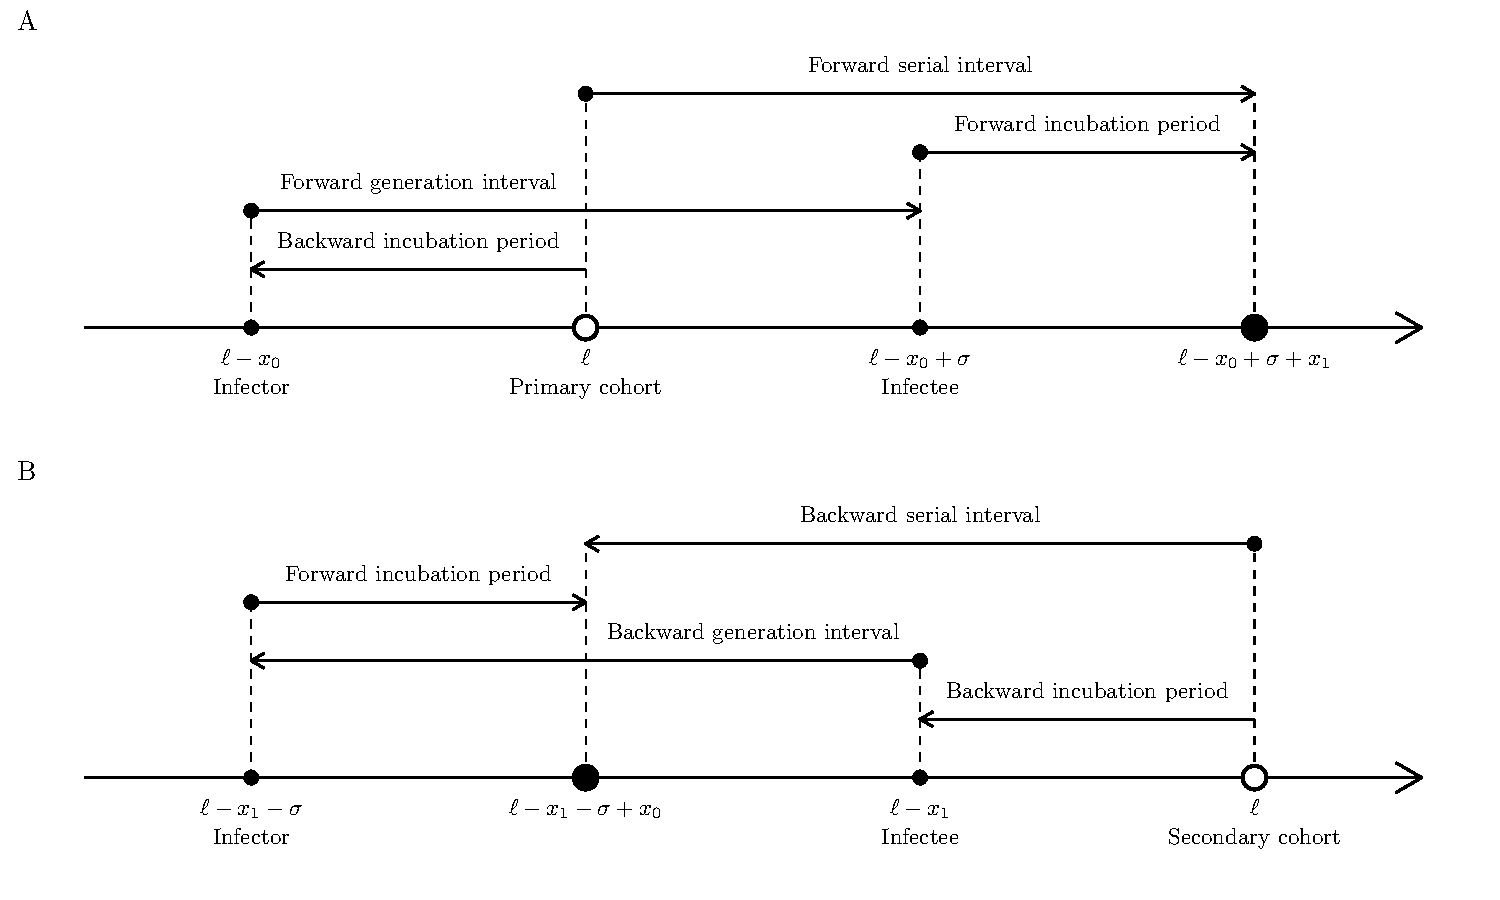
\includegraphics[width=\textwidth]{serial_guide.pdf}
\caption{\textbf{Illustration of intrinsic,
    forward and backward serial intervals.}  (A) The intrinsic serial
  interval for a cohort of individuals infected at time $\psymp$.  In
  this case, $\tau_{\rm i1}$ is drawn from the intrinsic incubation period
  distribution; $\gtime$ is drawn from the intrinsic generation-interval
  distribution; and $\tau_{\rm i2}$ is drawn from the intrinsic incubation period
  distribution.  (B) The forward serial interval for a cohort of
  infectors who became symptomatic at time $\psymp$.  In this case,
  $\tau_{\rm i1}$ is drawn from the backward incubation period distribution; $\gtime$
  is drawn from the forward generation-interval distribution; and $\tau_{\rm i2}$
  is drawn from the forward incubation period distribution.  (C) The
  backward serial interval for a cohort of infectees who became
  symptomatic at time $\ssymp$.  In this case, $\tau_{\rm i1}$ is drawn from the
  forward incubation period distribution; $\gtime$ is drawn from the
  backward generation-interval distribution; and $\tau_{\rm i2}$ is drawn from the
  backward incubation period distribution.}
\label{fig:diagram}
\end{figure}

To correctly link the realized serial interval distribution to the renewal process
between cases based on symptom onset dates, we must use the forward
serial interval (i.e., use the perspective of a cohort of infectors
that share the same symptom onset time).  Given that an infector
became symptomatic at time $\psymp$, to calculate the forward serial
interval we first go backward in time to when the infector was
infected, and then forward in time to when the infectee was infected,
and then forward to when the infectee became symptomatic.
In \fref{diagram}B, we see that $\tau_{\rm i1}$ is drawn from
the backward incubation period distribution of the cohort
of infectors who became symptomatic at time $\psymp$; $\gtime$ is drawn from
the forward generation-interval distribution of the cohort of
infectors who became infected at time $\psymp - \tau_{\rm i1}$; and $\tau_{\rm i2}$
is drawn from the forward incubation period distribution of the cohort of
infectees who became infected at time $\psymp - \tau_{\rm i1} + \gtime$.
Likewise, we can define the backward serial interval distribution for
a cohort of infectees who became symptomatic at time $\ssymp$
(\fref{diagram}C).  This conceptual framework demonstrates
that the distributions of $\tau_{\rm i1}$, $\gtime$, and $\tau_{\rm i2}$ (and therefore
the distributions of realized serial intervals) depend on the
reference cohort, which is defined by an event type (primary or secondary),
temporal direction (forward or backward), and a particular reference time.

To calculate realized serial-interval distributions, we begin by modeling $\total(\psymp,\ssymp)$: the total amount of serial intervals that start (when infectors develop symptoms) at time $\psymp$ and end (when infectees develop symptoms) at time $\ssymp$.
The amount of serial intervals between time $\psymp$ and $\ssymp$,
given that the infectors became infected at time $\pinf\le\psymp$ and
the infectees became infected at time $\sinf\le\ssymp$, depends on the
amount of infection that occurs between time $\pinf$ and $\sinf$ as
well as the density of forward incubation periods between $\pinf$ and
$\psymp$ (realized incubation periods of infectors) and between
$\sinf$ and $\ssymp$ (realized incubation periods of infectees):
\begin{equation}
\underbrace{\Rc (\pinf)}_{\substack{\text{case} \\ \text{reproduction} \\ \text{number}}} 
\times 
\underbrace{i(\pinf)}_{\text{incidence}} 
\times 
\underbrace{h_{\pinf}(\psymp-\pinf, \sinf - \pinf)}_{\substack{\text{joint density of} \\ \text{the forward incubation} \\ \text{period } p-\pinf \text{ and the forward} \\ \text{generation interval } \sinf-\pinf\\ \text{(of infectors)}}}
\times
\underbrace{\idist_{\sinf}(\ssymp - \sinf)}_{\substack{\text{marginal density of} \\ \text{the forward incubation} \\ \text{period } \ssymp-\sinf \\ \text{(of infectees)}}},
\end{equation}
where the case reproduction number $\Rc (\pinf)$ is defined as the average number of secondary cases caused by a primary case infected at time $\pinf$ over the course of their infection \citep{fraser2007estimating}.
We describe the forward incubation periods and the forward generation intervals using a joint probability distribution because onset of symptoms and transmission potential jointly depend on the life history of a disease;
for example, if an infected individual can only transmit the disease after symptom onset, the forward generation interval will necessarily be longer than the forward incubation period.

The total amount of serial intervals can now be obtained by integrating over all possible infection times for the infector and the infectee:
\begin{equation}
\total (\psymp,\ssymp) = \int_{-\infty}^{\psymp} \int_{\pinf}^{\ssymp} \Rc (\pinf) i(\pinf) h_{\pinf}(\psymp-\pinf, \sinf - \pinf) \idist_{\sinf}(\ssymp - \sinf) \, \mathrm{d}\sinf\,\mathrm{d}\pinf.
\end{equation}
Then, the forward serial-interval distribution $f_\psymp(\tau)$ is given by the density of intervals of length $\tau$ starting at \psymp, relative to the total number of serial intervals starting at \psymp: 
\begin{equation}
f_\psymp(\tau) = 
\frac{\total(\psymp, \psymp+\tau)}{\int_{-\infty}^\infty \total(\psymp, \psymp+\tau') \dtau'}.
\label{eq:fserial}
\end{equation}
Likewise, the backward serial-interval distribution $b_\ssymp(\tau)$ is given by the density of intervals of length $\tau$ ending at \ssymp, relative to the total number of serial intervals ending at \ssymp: 
\begin{equation}
b_\ssymp(\tau) = 
\frac{\total(\ssymp-\tau, \ssymp)}{\int_{-\infty}^\infty \total(\ssymp-\tau', \ssymp) \dtau'}.
\label{eq:bserial}
\end{equation}
This framework allows us to understand changes in the realized serial intervals for any deterministic epidemic model.

\subsection{Epidemic model}

We illustrate changes in the forward and backward serial intervals over the course of an epidemic by applying it to a specific example of an epidemic model. 
We model disease spread with a renewal-equation model \citep{heesterbeek1996concept, diekmann2000mathematical, roberts2004modelling, aldis2005integral, roberts2007model, champredon2018equivalence}.
Ignoring births and deaths, changes in the proportion of susceptible individuals $S(t)$ and incidence of infection $i(t)$ can be written as:
\begin{align}
\frac{\mathrm{d}S}{\mathrm{d}t} &= - i(t)\nonumber\\
i(t) &= \Ro S(t) \int_0^\infty i(t-\tau) \gdist(\tau) \dtau,
\label{eq:renewal}
\end{align}
where \Ro is the basic reproduction number, and $\gdist(\tau)$ is the intrinsic generation-interval distribution (i.e., the forward generation-interval distribution of a primary case in a population where the number of susceptibles remains constant).
Then, the forward generation-interval for a cohort of individuals that were infected at time $\psymp$ follows \citep{champredon2015intrinsic}:
\begin{equation}
\gdist_\psymp (\tau) = \frac{ \gdist(\tau) S(\psymp + \tau)}{\int_0^\infty \gdist(\tau') S(\psymp + \tau') \dtau'},
\end{equation}
which allows us to separate the joint probability distribution $h_\psymp$ of the forward incubation period and the forward generation-interval distribution as a product of the proportion of susceptible individuals $S$ and the joint probability distribution $h$ of the forward incubation period and the intrinsic generation intervals:
\begin{equation}
h_\psymp (x, \tau) = \frac{h(x, \tau) S(\psymp + \tau)}{\int_0^\infty \int_0^\infty h(x', \tau') S(\psymp + \tau') \dtau' \dx'}.
\end{equation}
We further assume that the forward incubation period distribution does
not vary across cohorts over the course of an epidemic, as it
represents the life history of a disease; we denote it as $\idist$.
Then, we have:
\begin{align}
\idist(x) &= \int_0^\infty h(x, \tau) \dtau\nonumber\\
\gdist(\tau) &= \int_0^\infty h(x, \tau) \dx
\label{eq:marginal}
\end{align}
Finally, the case reproduction for this model is defined as follows:
\begin{equation}
\Rc(t) = \Ro \int_0^\infty \gdist(\tau) S(t+\tau) \dtau.
\end{equation}
The forward and backward serial-interval distributions are then calculated by substituting these quantities into \eref{fserial} and \eref{bserial}.
We use this framework to illustrate how the realized epidemiological time distributions vary over the course of an epidemic and depend on the perspective (i.e., forward vs. backward).

\subsection{Linking $r$ and \RR}

During the initial phase of an epidemic, the proportion susceptible remains approximately constant ($S(t) \approx S(0)$) and incidence of infection grows exponentially: $i(t)=i_0\exp(rt)$.
During this period, the intrinsic generation-interval distribution provides the correct link between the exponential growth rate $r$ and the initial reproduction number $\RR=\Ro S(0)$ based on the Euler-Lotka equation \citep{wallinga2007generation};
in this case, we focus on the estimates of the basic reproduction number \Ro (the value of \RR in a fully susceptible population, $S(t) \approx 1$):
\begin{equation}
\frac{1}{\Ro} = \int_0^\infty \exp(-r\tau) g(\tau) \dtau.
\label{eq:Rgen}
\end{equation}
Analogous to the intrinsic generation-interval distribution, 
forward serial-interval distributions, by definition, describe the renewal process of infection based on symptom onset dates.
Therefore, we expect the forward serial-interval distribution during the exponential growth phase --- which we refer to as the \emph{initial} forward serial-interval distribution $f_0$ --- to estimate the same value of \Ro for a given $r$ as the intrinsic generation-interval distribution (note, however, that the forward serial interval is not necessarily positive):
\begin{equation}
\frac{1}{\Ro} = \int_{-\infty}^\infty \exp(-r\tau) f_{0}(\tau) \mathrm{d} \tau,
\label{eq:Rforward}
\end{equation}
where the initial forward serial-interval distribution is given by:
\begin{equation}
f_{0}(\tau) \propto \int_{-\infty}^{0} \int_{\pinf}^{\tau} \exp(r \pinf) h(-\pinf, \sinf - \pinf) \idist(\tau - \sinf) \, \mathrm{d}\sinf\,\mathrm{d}\pinf.
\label{eq:initialSI}
\end{equation}
In Supplementary Materials, we provide a mathematical proof of this relationship.
We further compare this with the estimate of \Ro based on the intrinsic serial-interval distribution $q(\tau)$:
\begin{equation}
\frac{1}{\Rintrinsic} = \int_{-\infty}^\infty \exp(-r\tau) q(\tau) \mathrm{d} \tau,
\label{eq:Rintrinsic}
\end{equation}
where the intrinsic serial-interval distribution $q(\tau)$ does not depend on epidemic dynamics:
\begin{equation}
q(\tau) \propto \int_{-\infty}^{0} \int_{\pinf}^{\tau} h(-\pinf, \sinf - \pinf) \idist(\tau - \sinf) \, \mathrm{d}\sinf\,\mathrm{d}\pinf.
\label{eq:intrinsicSI}
\end{equation}
Rather than numerically integrating over closed forms of $g$, $f_0$, and $q$ to estimate $\Ro$, we use simulation-based approaches for simplicity (Supplementary Materials).

The initial forward serial-interval distribution depends on the exponential growth rate $r$.
For a fast-growing epidemic (high $r$), we expect the backward incubation periods to be short (\eref{backexp}), and therefore, the forward serial-interval distribution will generally have a larger mean than the intrinsic generation- and serial-interval distributions.
The Susceptible-Exposed-Infected-Recovered model, under the additional assumption that the incubation and exposed periods are equivalent (i.e. that onset of symptoms and infectiousness occur simultaneously), provides a special case where the forward serial- and generation-intervals follow the same distributions during the exponential growth phase because (i) infected individuals can only transmit after symptom onset and (ii) the time between symptom onset to infection is independent of the incubation period of an infector (see Supplementary Materials).

\begin{table}[!th]
\begin{center}
\begin{tabular}{|l|l|r|}
\hline
Parameter & Values & Source\\
\hline
Mean intrinsic incubation period & 5.5 days & \cite{lauer2020incubation} \\
SD intrinsic incubation period & 2.4 days & \cite{lauer2020incubation} \\
Mean intrinsic generation interval & 5 days & \cite{ferretti2020quantifying} \\
SD intrinsic generation interval & 2 days & \cite{ferretti2020quantifying} \\
\hline
\end{tabular}
\end{center}
\caption{
  \textbf{Parameter values used for simulations.}
The intrinsic generation-interval distribution is parameterized using a log-normal distribution with log mean $\mu_G=1.54$ and log standard deviation $\sigma_G=0.37$.
The intrinsic incubation period distribution is parameterized using a log-normal distribution with log mean $\mu_I=1.62$ and log standard deviation $\sigma_I=0.42$.
The joint probability distribution is modeled using a multivariate log-normal distribution with correlations (on the log scale) $\rho=-0.5, 0, 0.5$.
The intrinsic generation-interval and incubation period distributions are chosen to match characteristic of COVID-19 to illustrate realistic magnitudes of time-varying/perspective effects in the current pandemic.
}
\end{table}

\section{Results}

\subsection{Realized serial interval distributions}

First, we compare the estimates of the basic reproduction number \Ro based on the initial forward serial-interval distributions and the intrinsic serial-interval distributions (see Supplementary Materials for calculation details.).
In particular, we model the joint probability distribution of the intrinsic incubation periods and generation intervals using a bivariate lognormal distribution with correlation $\rho$ based on parameter estimates for COVID-19 (Table 1).
The initial forward serial-interval distributions $f_0(\tau)$ and the intrinsic generation-interval distribution $\gdist(\tau)$ give identical estimates of \Ro (see \eref{Rgen} and \eref{Rforward}) regardless of the correlation $\rho$ between the intrinsic incubation period and the intrinsic generation interval (\fref{rR}A).
However, using the intrinsic serial-interval distributions that do not account for epidemic dynamics (i.e., assuming that the backward and the forward incubation period distributions are identical) underestimates \Ro (see \eref{Rintrinsic});
as $r$ increases, \Rintrinsic saturates and eventually decreases due to negative serial intervals (\fref{rR}B).
While the forward serial intervals during the exponential growth phase can also be negative, the proportion of negative intervals are appropriately balanced because faster epidemic growth will lead to shorter backward incubation periods (and therefore a lower proportion of negative serial intervals).

\begin{figure}[!th]
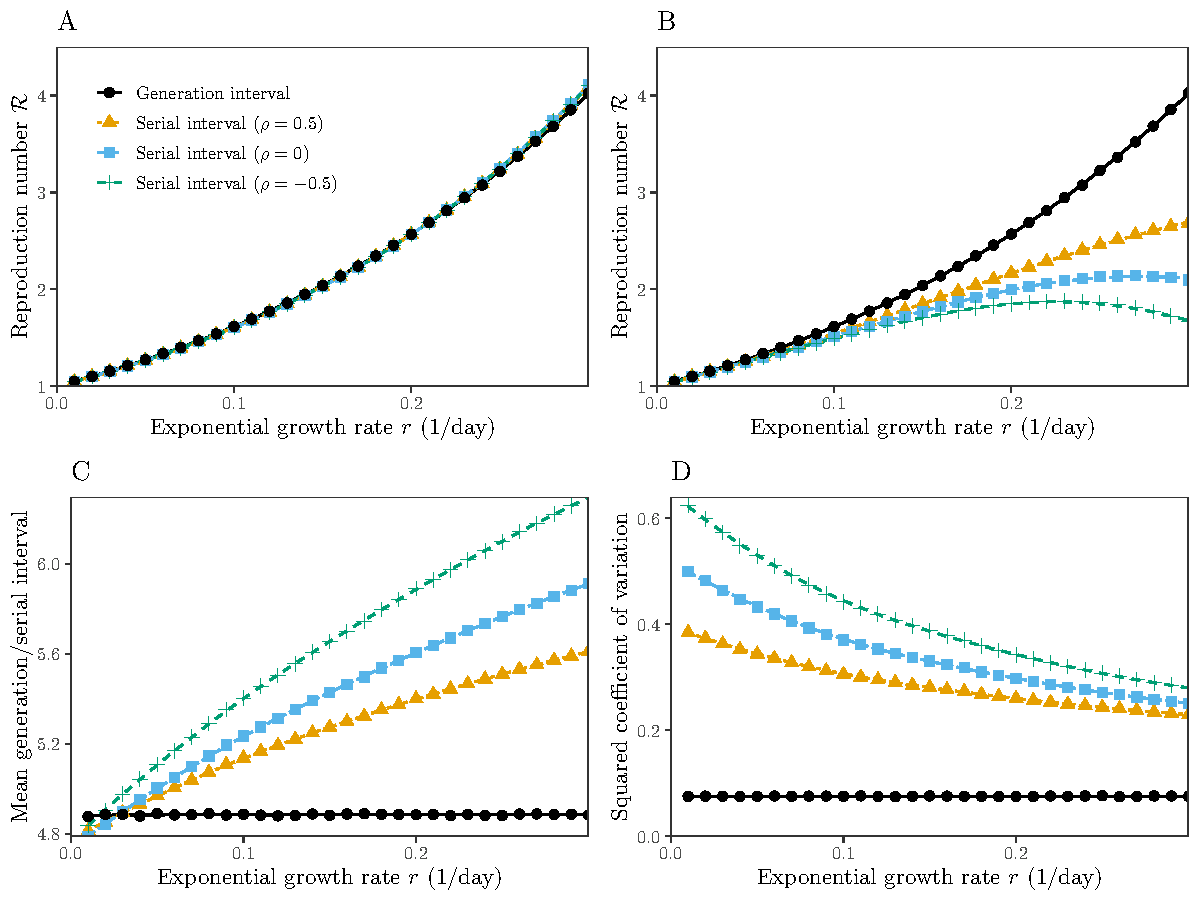
\includegraphics[width=\textwidth]{rR.pdf}
\caption{
\textbf{Estimates of the reproduction number from the exponential growth rate based on serial- and generation-interval distributions.}
(A). The initial forward serial-interval distributions give a correct
link between the exponential growth rate $r$ and the reproduction
number \Ro,
for any correlation $\rho$ between intrinsic incubation period and
intrinsic generation interval of the underlying bivariate log-normal distribution.
(B) The intrinsic serial-interval distributions give an incorrect link between $r$ and \Ro.
(C) The mean initial forward serial interval during the exponential growth phase increases with $r$.
(D) The squared coefficient of variation of the initial forward serial intervals during the exponential growth phase decreases with $r$.
}
\label{fig:rR}
\end{figure}

Comparing the shapes of the initial forward serial-interval distribution (\eref{initialSI}) and the intrinsic generation-interval distribution allows us to better understand how different forward distributions lead to identical estimates of \Ro.
In general, distributions with higher means and less variability lead to higher \Ro for a given $r$ \citep{wallinga2007generation, weitz2015modeling, park2019practical}.
When incidence is growing exponentially, forward serial intervals have higher means (\fref{rR}C) and squared coefficients of variation (\fref{rR}D) than the intrinsic generation-interval distribution.
The effects of higher means (which increase \Ro) exactly cancel those of higher variability (which decrease \Ro).
On the other hand, \emph{intrinsic} serial intervals (\eref{intrinsicSI}) have the same mean (equal to the mean initial forward serial at $r=0$ in \fref{rR}C) as the intrinsic generation intervals but are wider (also see squared coefficient of variation of the initial forward serials at $r=0$ in \fref{rR}D); 
therefore, we underestimate \Ro when we use the intrinsic serial-interval distribution.

\begin{figure}[!ht]
\begin{center}
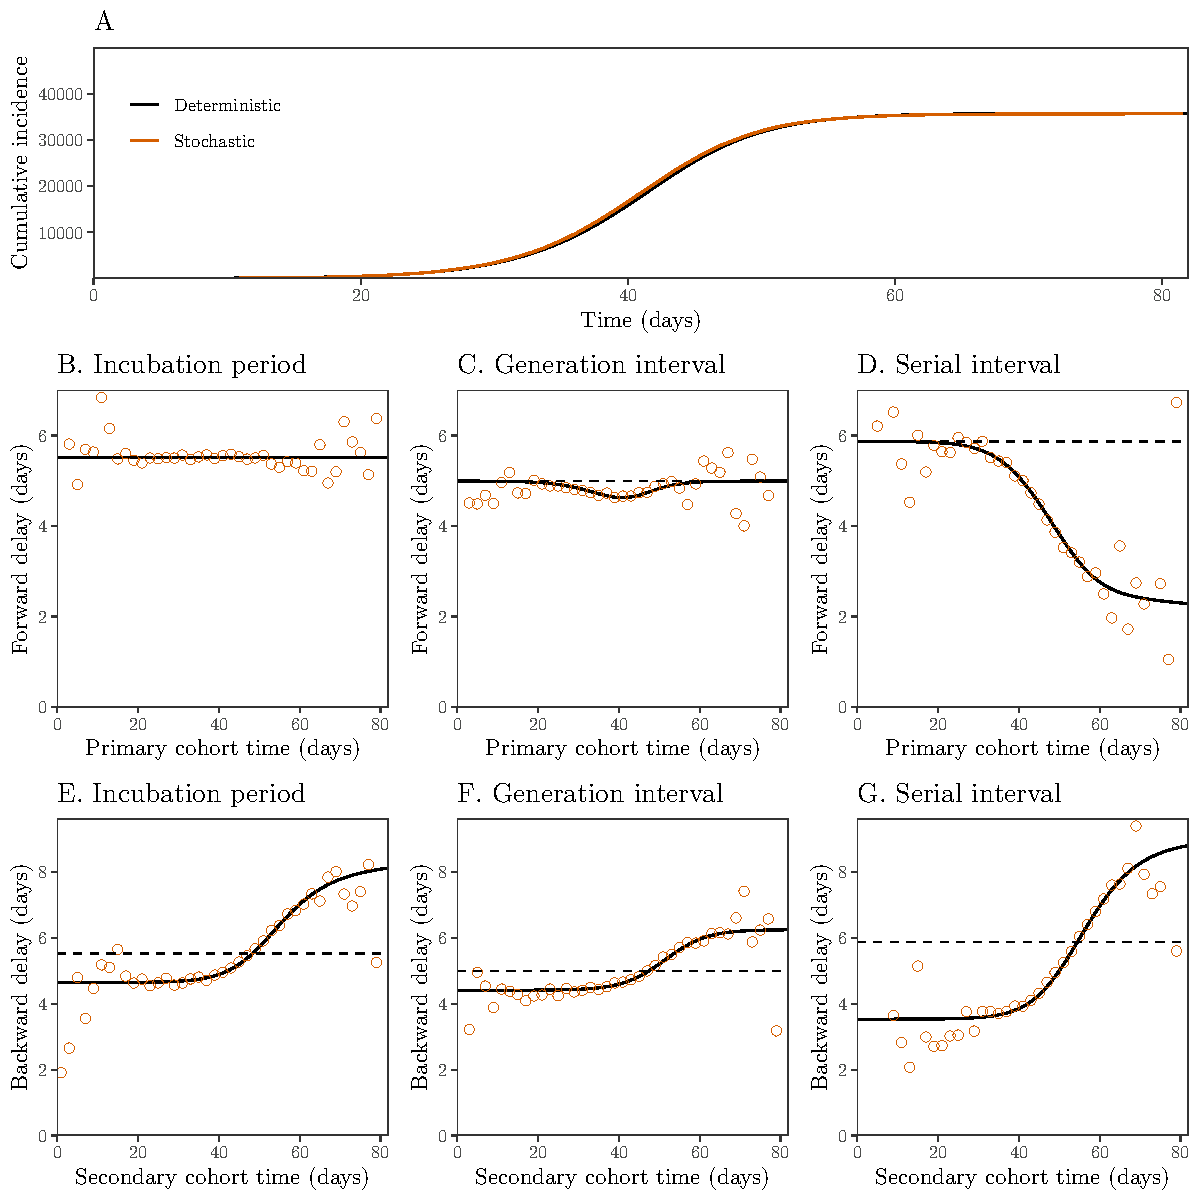
\includegraphics[width=0.95\textwidth]{forward.pdf}
\caption{
\textbf{Epidemiological dynamics and changes in mean forward and backward delay distributions.}
(A) Daily incidence over time.
(B--D) Changes in the mean forward incubation period, generation interval, and serial interval.
(E--G) Changes in the mean backward incubation period, generation interval, and serial interval.
Black lines represent the results of a deterministic simulation.
Orange lines (A) represent the results of 10 stochastic simulations.
Orange points (B-G) represent the average of 10 stochastic simulations.
Dashed lines represent the mean initial forward delay.
Intrinsic incubation periods and intrinsic generation-intervals are assumed to be independent of each other.
See Table 1 for parameter values.
}
\label{fig:epi}
\end{center}
\end{figure}

The initial forward serial interval distribution captures the exponential growth phase of an epidemic.
Next, we characterize how forward and backward serial intervals vary over the course of an epidemic by running deterministic and stochastic simulations based on the renewal equations (see Supplementary Materials) using parameters in Table 1;
we further assume $\Ro=2.5$.
While the forward serial-interval distribution is our primary focus, understanding the differences between the forward and the backward distributions is important because the observed intervals during an ongoing epidemic are often the backward ones:
we typically identify infected individuals and ask when and by whom they were infected.
Similarly, when we are estimating the incubation period of an individual, we typically observe their symptom onset date and try to estimate when they were infected (e.g., \cite{backer2020incubation}).

\fref{epi} shows the epidemiological dynamics (A) together with the mean forward (B--D) and the mean backward (E--F) delay distributions of a deterministic model based on the renewal equation (\eref{renewal}) and of the corresponding stochastic realizations based on individual-based simulations.
The mean forward incubation period remains constant throughout an epidemic as assumed (\fref{epi}B).
The mean forward generation interval decreases slightly as incidence increases, causing the proportion of susceptible population to decrease (\fref{epi}C; \cite{kenah2008generation, champredon2015intrinsic}).
In contrast, the mean forward serial interval decreases over time (\fref{epi}D).

The forward serial interval distributions depend on distributions of three intervals
(\fref{diagram}): (i) the backward incubation period, (ii) the forward generation interval, and (iii) the forward incubation period.
For COVID-19 parameters (Table 1), both forward incubation period (\fref{epi}B) and generation-interval (\fref{epi}C) distributions remain roughly constant;
therefore, changes in the forward serial-interval distributions are predominantly driven by changes in the backward incubation period distributions, whose mean increases over time (\fref{epi}D).
In this case, the increase in the mean backward incubation period directly translates to the decrease in the mean forward serial interval.
% Since the increase in the mean backward period is driven by the decreasing incidence, which can still occur in the absence of significant depletion of the susceptible pool via intervention, decrease in the mean forward serial interval may be a robust feature in COVID-19 outbreaks.
In general, relative contributions of the three distributions depend on their shapes, correlations between intrinsic incubation periods and generation intervals, and overall epidemiological dynamics.

We see similar qualitative patterns in all three backward delays (\fref{epi}E--G; \eref{backward}), because they are predominantly driven by the rate of change in incidence, which in turn affects relative cohort sizes.
When incidence is increasing, individuals are more likely to have been infected recently and therefore, we are more likely to observe shorter intervals (\eref{backexp}).
Similarly, when incidence decreases, we are more likely to observe longer intervals.
Neglecting these changes in the backward distributions will necessarily bias the inference of the intrinsic distributions from the observed distributions.

\subsection{Observed serial interval distributions}

\begin{figure}[!ht]
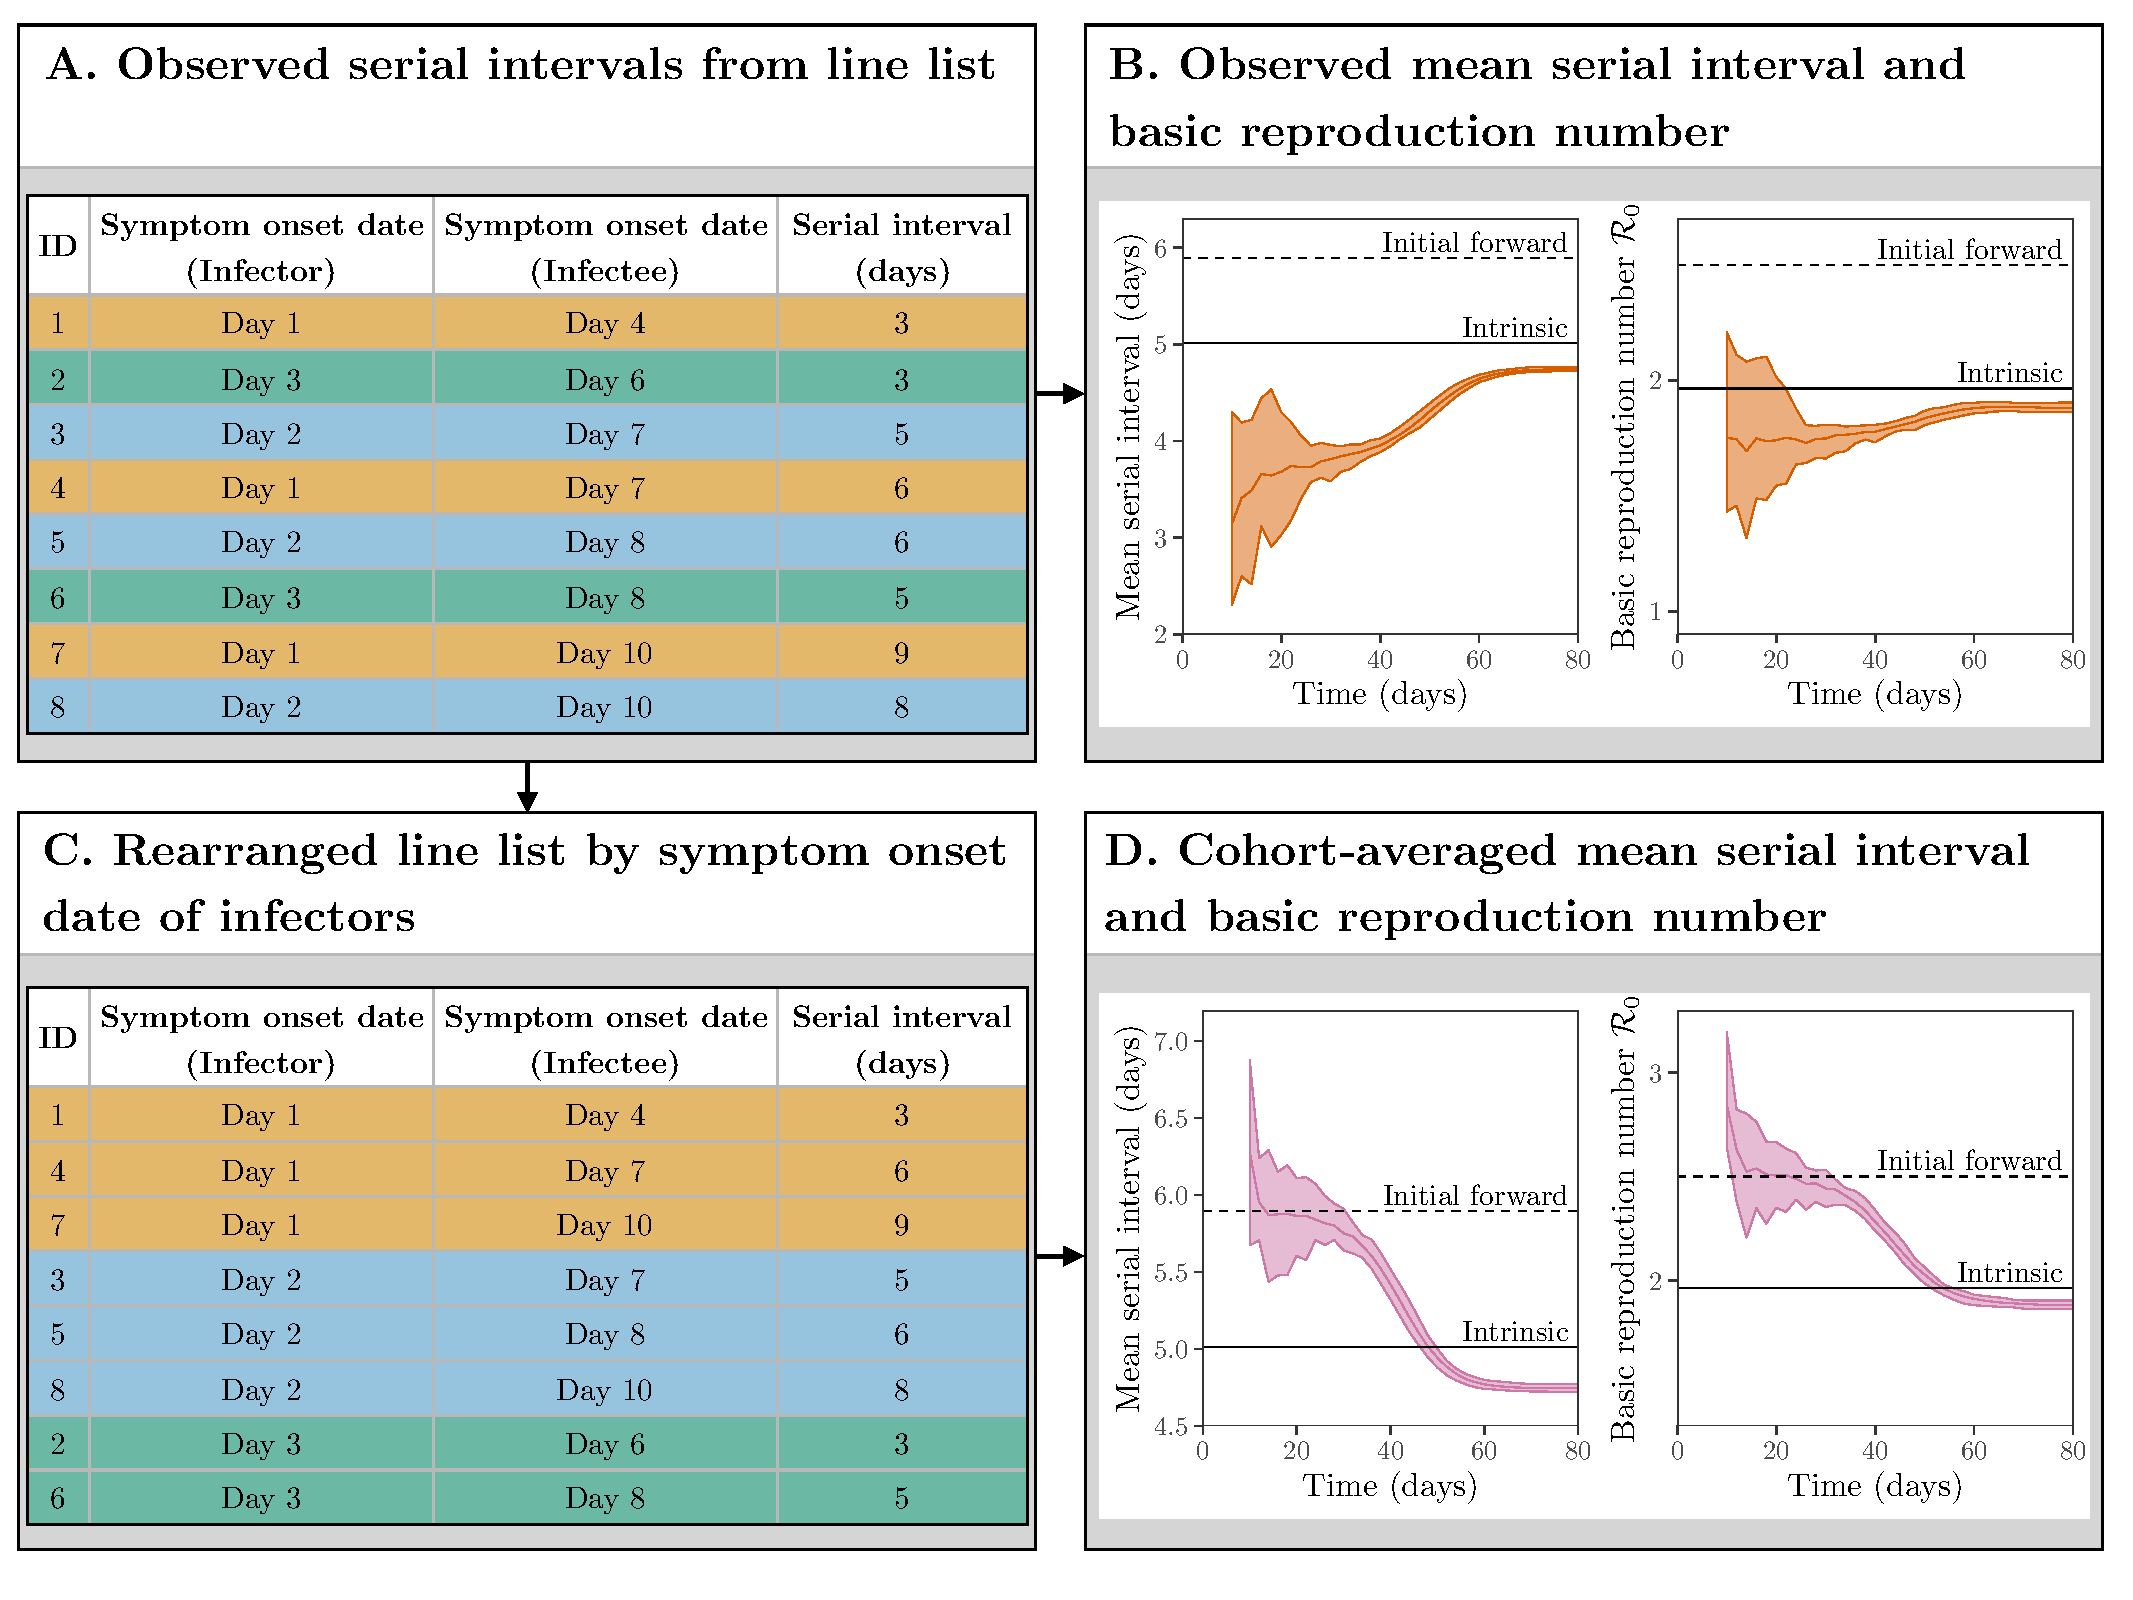
\includegraphics[width=\textwidth]{diagram.pdf}
\caption{
\textbf{Estimating the reproduction number from the observed serial intervals.}
(A) Schematic representation of line list data collected during an epidemic.
(B) Estimates of \Ro based on all observed serial intervals completed by a given time.
(C) Schematic representation of line list data rearranged by symptom onset date of infectors.
(D) Estimates of \Ro based on all observed serial intervals started by a given time. 
Black dashed lines represent the mean initial forward serial interval and \Ro.
Black solid lines represent the mean intrinsic serial interval and \Rintrinsic.
Colored solid lines represent the mean estimates of \Ro across 10 stochastic simulations.
Colored ribbons represent the range of estimates of \Ro across 10 stochastic simulations.
}
\label{fig:obsrR}
\end{figure}

Now, we turn to issues of estimating the reproduction number from the observed serial interval data during on ongoing epidemic.
In order to have an unbiased estimate of the basic reproduction number, we need to use serial-interval distributions estimated based on primary cohorts (i.e., infectors who share the same symptom onset time) at the early stage of the epidemic (i.e., initial forward serial-interval distribution).
However, researchers typically use all available information to estimate epidemiological parameters;
in particular, \cite{thompson2019improved} recently suggested that up-to-date serial interval data are necessary to accurately estimate the reproduction number.
We explore the consequences of neglecting changes in the realized serial interval distribution on estimates of the basic reproduction number.

When an epidemic is ongoing, the observed serial intervals are subject to right-censoring because we cannot observe a serial interval if either an infector or an infectee has not yet developed symptoms;
for example, if we were to measure serial intervals on Day 8 as in \fref{obsrR}A, we will only be able to observe the first 6 events (ID 1--6).
\fref{obsrR}B demonstrates how the effect of right-censoring in the observed serial intervals translates to the underestimation of the basic reproduction number \Ro in our stochastic simulations (assuming $\Ro = 2.5$ as in \fref{epi}).
Notably, even if we could observe, and average, \emph{all} serial intervals across all transmission pairs after the epidemic has ended, we would still underestimate the initial mean forward serial interval (and therefore \Ro), likely by a large amount, because the observed serial-interval distribution converges to the intrinsic serial-interval distribution;
in fact, we would even underestimate the intrinsic value slightly due to contraction of the forward generation-interval distribution during the susceptible depletion phase (\fref{epi}C).

Here we provide a heuristic way of assessing potential biases in the estimate of the mean initial forward serial interval and therefore \Ro retrospectively.
We can rearrange the line list and group observed serial intervals based on the symptom onset date of infectors (\fref{obsrR}C).
Then, we can compare how estimates of the mean serial interval as well as \Ro change as we incorporate more recent cohorts into the analysis;
that is, we analyze observed serial intervals from infectors who became symptomatic before time $t$ and evaluate how the estimates change as we increase $t$.
This approach is analogous to averaging over a set of forward intervals, just as using all information up to a certain time is analogous to averaging over a set of backward intervals (\fref{obsrR}D).
During the exponential growth phase, the estimates of the mean serial interval and \Ro are consistent with the true value (see `initial forward' in \fref{obsrR}B,D);
adding more data allows us to make more precise inference during this period.
However, the cohort-averaged estimates decrease rapidly soon after the exponential growth period, reflecting changes in the forward serial-interval distributions.
This approach allows us to detect dynamical changes in the forward serial-interval distributions and its effect on the estimates of \Ro.

\subsection{Applications to the COVID-19 pandemic}

\begin{figure}[!th]
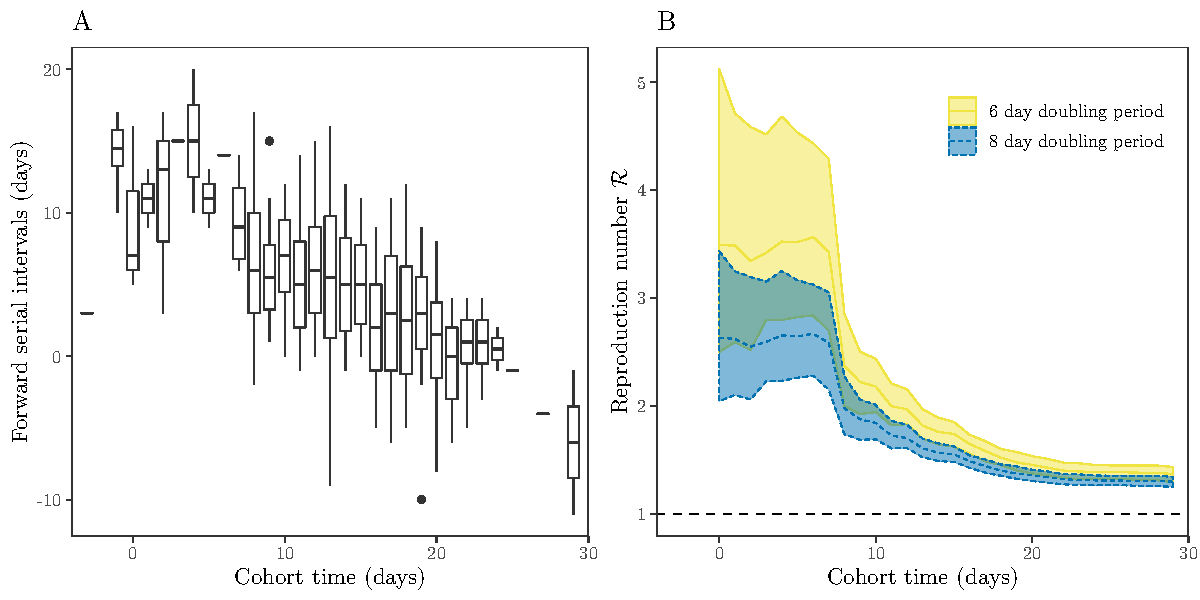
\includegraphics[width=\textwidth]{serial_analysis.pdf}
\caption{
\textbf{Observed serial intervals of COVID-19 and cohort-averaged estimates of \RR.}
(A--B) forward and backward serial intervals over time.
Points represent the means. 
Vertical error bars represent the 95\% equi-tailed quantiles.
Solid lines represent the estimated locally estimated scatterplot smoothing (LOESS) fits.
The dashed line represents the maximum and minimum observable delays across the range of reported sypmtom onset dates.
(C) Cohort-averaged estimates of \Ro assuming doubling period of 6 and 8 days \citep{li2020early, wu2020nowcasting}.
Ribbons represent the associated 95\% bootstrap confidence intervals.
The data were taken from Supplementary Materials of \cite{du2020serial}.
}
\label{fig:du}
\end{figure}

Finally, we re-analyze serial intervals of COVID-19 collected by \cite{du2020serial} from mainland China, outside Hubei province, based on transmission events reported between January 21--February 8, 2020;
\cite{du2020serial} estimated the mean serial interval of 3.96 days (95\% CI 3.53–4.39 days) and \Ro of 1.32 (95\% CI 1.16–1.48).
\fref{du}A shows that the mean forward serial interval decreases over time.
While the decrease is likely to be affected by the right-censoring (indicated by the closeness between the quantiles of the observed serial intervals and maximum observable serial intervals), the increase in the proportion of negative serial intervals unequivocally indicates changes in the forward serial-interval distribution;
the increase in the proportion of negative intervals is unlikely to be driven by left-censoring (indicated by the distance between the quantiles of the observed serial intervals and minimum observable serial intervals).
The decrease in the mean forward serial interval was probably caused by increase in the mean backward incubation period, reflecting decrease in COVID-19 cases in China, as well as intervention efforts which reduced generation intervals by preventing infections once cases were identified.
\fref{du}B shows that the mean backward serial interval increased over time, also reflecting decrease in COVID-19 cases in China.

While the qualitative changes in the mean forward and backward serial interval are consistent with our earlier simulations (\fref{epi}), the initial mean forward serial interval (\fref{du}A) appears to be larger than what we calculate earlier based on previously estimated incubation period and generation-interval distributions (\fref{rR}C).
These results indicate that the incubation period and generation interval (Table 1) may previously have been underestimated as neither study explicitly accounted for the fact that the observed intervals were drawn from the backward distributions and were likely to have been truncated.

\fref{du}C shows the cohort-averaged estimates of \Ro, which remain roughly constant until day 7 and suddenly decreases;
this sudden decrease is indicative of changes in the forward serial intervals as shown in our simulation study (\fref{obsrR}).
The cohort-averaged estimates of \Ro based on the early forward serial intervals are also consistent with previous estimates of \Ro of the COVID-19 epidemic in China \citep{majumder2020early, park2020reconciling}:
$\Ro = 2.6$ (95\% CI: 2.2--3.1) and $\Ro = 3.4$ (95\% CI: 2.7 -- 4.3) based on 8 and 6 doubling periods, respectively, using serial interval data from infectors who developed symptoms by day 7.
These early cohort-averaged estimates of \Ro are unlikely to be affected by the right-censoring as we expect the degree of right-censoring to be low (\fref{du}A).
Therefore, the \Ro estimate of 1.32 (95\% CI 1.16–1.48), which neglects the changes in the forward serial-interval distribution, is likely to be an underestimate.
This example demonstrates the danger of using the observed serial intervals to calculate the reproduction number without integrating serial intervals into cohorts.

\section{Discussion}

Generation and serial intervals determine the time scale of disease transmission, and are therefore critical to dynamical modeling of infectious outbreaks.
Here, we show that the initial \emph{forward} serial-interval distribution --- measured during the exponential growth phase of an epidemic --- provides the correct link between the exponential growth rate $r$ and the reproduction number \RR.
In general, the forward serial-interval distributions will not match the intrinsic or the backward serial-interval distributions.
Further, the mean forward serial interval can decrease over time due to epidemic dynamics. 
Failing to account for these differences can result in underestimation of \RR.

Our study underlines the importance of carefully defining measured epidemiological time distributions.
Previous studies have shown that it matters whether generation
intervals are measured forward or backward \citep{nishiura2010time,champredon2015intrinsic,britton2019estimation};
we generalize these ideas and show that they apply to other epidemiological distributions.
Changes in the backward delay distributions due to changing cohort sizes are expected to be a pervasive feature of outbreak dynamics.
Recent analyses of COVID-19 epidemics have attempted to reconstruct epidemic time series of symptomatic cases or infected cases from the reports of confirmed cases by using time-independent delay distributions from infection or symptom onset to reporting (e.g., \cite{tempvar, park2020potential, shim2020transmission});
these studies effectively assume constant backward delay distributions.
Although such approaches may be able to roughly match the time scale of an epidemic, we recommend using dynamical approaches that model incidence as well as reporting delays explicitly (e.g., \cite{flaxman2020estimating}).

While our results support the use of serial interval distributions for calculating \RR, 
they also reveal gaps in current practices in incorporating serial-interval distributions into outbreak analyses.
\cite{thompson2019improved} recently emphasized the importance of using up-to-date serial interval data for accurate estimation of time-varying reproduction numbers.
However, our study demonstrates that early serial interval data is required to estimate the initial \RR during the exponential growth phase and that using up-to-date serial interval data (without accounting for changes in the forward serial-interval distribution) can, in fact, underestimate the initial \RR.
Future studies should explore how neglecting changes in the forward serial-interval distribution can affect the estimates of \RR beyond the exponential growth phase and potentially re-assess existing estimates of \RR.

Many studies have already estimated the (time-varying) reproduction numbers for COVID-19 epidemics using aggregated serial interval data (e.g., \cite{tempvar,du2020serial,pan2020jama,zhang2020evolving});
these studies should also re-assess whether they appropriately considered the \emph{forward} serial interval.
Given large geographical variation in the spread of the COVID-19, the forward serial interval distributions are also likely to vary across countries.
We suggest that modelers should aim to characterize spatiotemporal variation in forward serial-interval distributions and understand their changes over time.
These modeling approaches should be necessarily coupled with intensive
epidemiological investigation through contact tracing at the very
beginning of the outbreak in order to characterize the initial forward
serial-interval distribution, particularly for an epidemic of an
emerging disease such as COVID-19.

Our study also underlines the fact that the serial-interval distribution depends not only on the generation-interval and incubation-period distributions, but also on their intrinsic correlations.
This implies that not considering this correlation can bias the estimates of the intrinsic generation-interval distribution from the serial-interval distribution.
Furthermore, previous studies that tried to estimate the generation-interval distributions from the observed serial intervals often ignored the dynamical differences between the realized incubation periods of infectors (backward-looking) and those of infectees (forward looking) (e.g., \cite{klinkenberg2011correlation, ganyani2020estimating}).
Better statistical tools for teasing apart the intrinsic generation-interval distributions from the observed serial intervals are needed.

Our study has some limitations.
We assumed that all individuals develop symptoms and that the entire transmission process, including all relevant epidemiological delays, is known exactly.
In practice, asymptomatic and presymptomatic transmission of COVID-19 makes measuring serial intervals difficult \citep{bai2020presumed,he2020temporal,wei2020presymptomatic}.
Biases in the observed serial intervals will necessarily bias the estimates of \RR. 
Furthermore, serial intervals do not take into account asymptomatic transmission; 
neglecting asymptomatic transmission may also bias the estimates of \RR \citep{park2020time}.

While we focused on the effect of epidemiological dynamics on the serial-interval distributions, other factors, such as intervention strategies, can also affect the generation- and serial-interval distributions.
Individual-level interventions, such as case isolation, and behavioral responses directly affect individuals' ability to transmit and will shorten the forward generation- and serial-intervals.
Population-level interventions, such as social distancing, can squeeze contacts into household and induce clustering, which will in turn shorten the realized generation interval due to local depletion of the susceptible pool within households \citep{park2019inferring}.

Despite these limitations, our analysis of serial intervals of COVID-19 from China provides further support for our theoretical framework, demonstrating temporal variation in serial intervals and its effect on the estimates of \RR.
Most existing estimates of the serial-intervals of COVID-19 implicitly or explicitly assume that the serial-interval distributions remain constant throughout the course of an epidemic \citep{du2020serial, he2020temporal, nishiura2020serial,tindale2020transmission,zhao2020estimating,zhang2020evolving}.
Our study provides a rationale for reassessing estimates of
serial-interval distributions---and their use in estimating
\RR---during the COVID-19 pandemic.

\pagebreak

\section{Supplementary Materials}

\subsection{Deterministic simulation}

We simulate the renewal equation model using a discrete-time approximation:
\begin{align}
i(t) &= \Ro S(t-\Delta t) \sum_{m=1}^{\tsub{m}{max}} i(t-m \Delta t) \hat{\gdist}(m \Delta t) \nonumber \\
S(t) &= S(t-\Delta t) - i(t)
\end{align}
where $\hat{\gdist}$ is a discrete-time intrinsic generation-interval distribution that satisfies the following:
\begin{equation}
\hat{\gdist}(m \Delta t) = \frac{\gdist(m \Delta t)}{\sum_{i=1}^\ell \gdist(m \Delta t)}, \quad m=1, \dots, \tsub{m}{max}.
\end{equation}
The continuous-time intrinsic generation-interval distribution is parameterized using a log-normal distribution (Table 1). We define the intrinsic incubation period distribution in a similar manner:
\begin{equation}
\hat{\idist}(m \Delta t) = \frac{\idist(m \Delta t)}{\sum_{i=1}^\ell \idist(m \Delta t)}, \quad m=1, \dots, \tsub{m}{max},
\end{equation}
where its continuous-time analog is also based on a log-normal distribution.
For simplicity, we assume that the forward incubation periods and intrinsic generation intervals are independent:
\begin{equation}
\hat{h}(m \Delta t, n \Delta t) = \hat{\idist}(m \Delta t)\hat{\gdist}(n \Delta t), \quad m,n=1, \dots, \tsub{m}{max}.
\end{equation}
We use $\Delta t = 0.025\,\textrm{days}$ and $\tsub{m}{max}=2001$ for discretization steps.

We initialize the simulation with population size $N$=40,000 as follows:
\begin{align}
i(m \Delta t) &= C \exp(r m \Delta t), \quad m=1, \dots, \tsub{m}{max}\nonumber \\
S(m \Delta t) &= N - \sum_{n=1}^m i(n \Delta t), \quad m=1, \dots, \tsub{m}{max}
\end{align}
where $C$ is chosen such that $\sum_{n=1}^{\tsub{m}{max}} i(m \Delta t)=10$.
These initial conditions allow the model to follow exponential growth from time $\Delta t (\tsub{m}{max} + 1)$ without any transient behaviors.
Results presented in the main text show simulations beginning from time $\Delta t (\tsub{m}{max} + 1)$.

\subsection{Stochastic simulation}

We run stochastic simulations of the renewal equation model using an individual-based model on a fully connected network (i.e., homogeneous population) based on the Gillespie algorithm that we developed earlier \citep{park2019inferring}.
First, we initialize an epidemic with $I(0)$ infected individuals (nodes) in a fully connected network of size $N$. 
For each initially infected individual, we draw number of infectious contacts from a Poisson distribution with the mean of \Ro and the corresponding generation intervals for each contact from a log-normal distribution (Table 1).
Contactees are uniformly sampled from the total population.
All contactees are sorted into event queues based on their infection time.
We update the current time to the infection time of the first person in the queue.
Then, the first person in the queue makes contacts based on the Poisson offspring distribution described earlier and their contactees are added to the sorted queue.
Whenever contactees are added to the sorted queue, we remove all duplicated contacts (but keep the first one) as well as contacts made to individuals that have already been infected.
Simulations continue until there are no more individuals in the queue.
We simulate 10 epidemics with $I(0)=10$ and $N$=40,000.

\subsection{Linking $r$ and \Ro using serial-interval distributions}

The intrinsic generation-interval distribution $\gdist(\tau)$ provides a link between $r$ and \Ro via the Euler-Lotka equation \citep{wallinga2007generation}:
\begin{equation}
\frac{1}{\Ro} = \int_0^\infty \exp(-r\tau) \gdist(\tau) \dtau\,.
\end{equation}
In this section, we prove that the initial forward serial-interval distribution $f_0(\tau)$ also estimates the same \Ro from $r$, except that integral extends to $\tau=-\infty$ rather than beginning at $\tau=0$, because serial intervals can be negative:
\begin{equation}
\frac{1}{\Ro} = \int_{-\infty}^\infty \exp(-r\tau) f_{0}(\tau) \dtau\,.
\label{eq:ptarget}
\end{equation}
Here, the initial forward serial-interval distribution $f_{0}(\tau)$ is defined as:
\begin{equation}
f_{0}(\tau) = \frac{1}{\phi} \int_{-\infty}^{0} \int_{\alpha_1}^{\tau} \exp(r \alpha_1) h(-\alpha_1, \alpha_2 - \alpha_1) \idist(\tau - \alpha_2) \, \mathrm{d}\alpha_2\,\mathrm{d}\alpha_1\,,
\label{eq:fdist}
\end{equation}
where $h$ is the joint probability distribution describing the
intrinsic generation-interval distribution $g$ and the intrinsic
incubation period distribution $\idist$ (see \eref{marginal} in the
main text), and the normalization constant $\phi$ is determined by the
requirement that $\int_{-\infty}^\infty f_{0}(\tau)\,\dtau=1$.

In order to verify \eref{ptarget}, we first rewrite the integral in \eref{fdist} by substituting $-\alpha_1$ for $\alpha_1$, and then changing the order of integration:
\begin{align}
f_{0}(\tau) &= \frac{1}{\phi} \int_0^\infty \int_{-\pinf}^{\tau} \exp(-r\pinf) h(\pinf, \sinf + \pinf) \idist(\tau - \sinf)\, \mathrm{d}\sinf\,\mathrm{d}\pinf\,,\nonumber \\
&= \frac{1}{\phi} \int_{-\infty}^{\tau} \int_{\max{(0,-\sinf)}}^{\infty} \exp(-r\pinf) h(\pinf, \sinf + \pinf)\idist(\tau - \sinf)\,\mathrm{d}\pinf\, \mathrm{d}\sinf\,.
\label{eq:newforward}
\end{align}
To further simplify the expression, we define $z(\sinf)$ as follows:
\begin{equation}
z(\sinf) = \int_{\max{(0,-\sinf)}}^{\infty} \exp(-r\pinf) h(\pinf, \sinf + \pinf) \,\mathrm{d}\pinf\,.
\end{equation}
Substituting $z(\sinf)$ into \eref{newforward} we obtain:
\begin{equation}
f_{0}(\tau) = \frac{1}{\phi} \int_{-\infty}^{\tau} z(\sinf) \idist(\tau - \sinf) \,\mathrm{d}\sinf\,,.
\end{equation}
Writing $\hat{z}$ for a normalized version of $z$,
\begin{equation}\hat{z}(\sinf) = \frac{z(\sinf)}{\int_{-\infty}^\infty z(x) \dx}\,,\end{equation}
we can now express the initial forward serial-interval distribution
$f_0$ as a convolution of $\hat{z}$ and $\idist$:
\begin{equation}
f_{0}(\tau) = \frac{1}{\hat{\phi}} \int_{-\infty}^{\tau} \hat{z}(\sinf) \idist(\tau - \sinf)\, \mathrm{d}\sinf\,,
\end{equation}
where $\hat{\phi} = \phi/\int_{-\infty}^\infty z(x) \dx$.

Since the right hand side of \eref{ptarget} is also a
Laplace transform of $f_0=\hat{z}*\idist$, we can express it as the product
of Laplace transforms of $\hat{z}$ and $\idist$:
\begin{equation}
\int_{-\infty}^\infty \exp(-r\tau) f_{0}(\tau) \mathrm{d} \tau = \int_{-\infty}^\infty \exp(-r\tau) \hat{z}(\tau)\, \mathrm{d} \tau \int_{0}^\infty \exp(-r\tau) \idist(\tau) \dtau\,.
\label{eq:newtarget}
\end{equation}
In order to derive an expression for a Laplace transform of $\hat{z}$, we have to first derive an analytical expression for $\int_{-\infty}^\infty z(x) \dx$. By changing the order of integration, we have:
\begin{align}
\int_{-\infty}^\infty z(\sinf) \mathrm{d}\sinf &= \int_{-\infty}^\infty \int_{\max{(0,-\sinf)}}^{\infty} \exp(-r\pinf) h(\pinf, \sinf + \pinf)\, \mathrm{d}\pinf \,\mathrm{d}\sinf\nonumber\,,\\
&= \int_{0}^\infty \int_{-\pinf}^\infty \exp(- r \pinf) h(\pinf, \sinf+\pinf)\, \mathrm{d}\sinf\,\mathrm{d} \pinf\,.
\end{align}
Since $\idist$ is a marginal probability distribution of $h$, it follows that:
\begin{equation}
\int_{-\infty}^\infty z(\sinf) \mathrm{d}\sinf = \int_{0}^\infty \exp(- r \pinf) \idist(\pinf)\, \mathrm{d}\pinf\,.
\end{equation}
Then, we have:
\begin{equation}
\hat{z}(\sinf) = \frac{\int_{\max{(0,-\sinf)}}^{\infty} \exp(-r\pinf) h(\pinf, \sinf + \pinf)\, \mathrm{d}\pinf}{\int_{0}^\infty \exp(- r \pinf) \idist(\pinf)\, \mathrm{d}\pinf}\,.
\end{equation}
Substituting the expression into \eref{newtarget}, we have:
\begin{equation}
\int_{-\infty}^\infty \exp(-r\tau) f_{0}(\tau)\dtau = \int_{-\infty}^\infty \exp(-r\sinf) \int_{\max{(0,-\sinf)}}^{\infty} \exp(-r\pinf) h(\pinf, \sinf + \pinf)\, \mathrm{d}\pinf\,\mathrm{d}\sinf\,.
\label{eq:newtarget2}
\end{equation}

Recall that $g$ is also a marginal probability distribution of $h$:
\begin{equation}
g(\tau) = \int_0^\infty h(x, \tau) \,\mathrm{d}x\,.
\end{equation}
We can then substitute $\tau = \pinf + \sinf$ into \eref{newtarget2} and apply change of variables to obtain:
\begin{align}
&\int_{-\infty}^\infty \exp(-r\tau) f_{0}(\tau)\dtau\\
&=\int_{-\infty}^{\infty} \exp(-r\sinf) \int_{\max(0, -\sinf)}^\infty \exp(- r \pinf) h(\pinf, \sinf+\pinf) \,\mathrm{d} \pinf \,\mathrm{d}\sinf \\
&=\int_{0}^{\infty} \int_{0}^\infty \exp(- r \tau) h(\pinf, \tau)\, \mathrm{d} \pinf\, \mathrm{d}\tau\\
&=\int_{0}^{\infty} \exp(-r\tau) g(\tau) \dtau =\frac{1}{\Ro}
\end{align}
Therefore, the initial forward serial-interval distribution and the intrinsic generation-interval distribution give the same estimates of \Ro from $r$.\qed

\subsection{Comparing the estimates of \Ro using the initial forward and the intrinsic serial-interval distributions}

We use a simulation-based approach to compare the estimates of \Ro based on the serial- and generation-interval distributions. 
To do so, we model the intrinsic generation-interval distribution and the incubation period using a multivariate log-normal distribution with log means $\mu_G, \mu_I$, log standard variances $\sigma_G^2, \sigma_I^2$, and log-scale correlation $\rho$;
the multivariate log-normal distribution is parameterized based on parameter estimates for COVID-19 (Table 1).
We construct forward serial intervals during the exponential growth period as follows:
\begin{equation}
F_i = -X_{1,i} + (G_i|X_{1,i}) + X_{2,i},
\end{equation}
where the backward incubation period $X_{1,i}$ of an infector is simulated by drawing random log-normal samples $Y_i$ with log mean $\mu_I$ and log variance $\sigma_I^2$ and resampling $Y_i$, each weighted by the inverse of the exponential growth function $\exp(-rY_i)$;
the intrinsic generation interval conditional on the incubation period of the infector $(G_i|X_{1,i})$ is drawn from a log-normal distribution with log mean $\mu_G + \sigma_G \rho (\log(X_{1,i}) - \mu_I)/\sigma_I$ and log variance $\sigma_G^2 (1-\rho^2)$;
the forward incubation period $X_{2,i}$ of an infectee is drawn from a log-normal distribution with log mean $\mu_I$ and log variance $\sigma_I^2$.
We then calculate the basic reproduction number \Ro using the empirical estimator:
\begin{equation}
\Ro = \frac{1}{\frac{1}{N}\sum_{i=1}^N \exp(- r F_i)}.
\end{equation}
We compare this with an estimate of \Ro based on the intrinsic serial-interval distribution which has the same mean as the intrinsic generation-interval distribution \citep{svensson2007note,klinkenberg2011correlation,champredon2018equivalence, britton2019estimation}:
\begin{equation}
  \Rintrinsic = \frac{1}{\frac{1}{N}\sum_{i=1}^N \exp(- r Q_i)},
\end{equation}
where
\begin{equation}
Q_i = -Y_i + (G_i|Y_i) + X_{2,i}.
\end{equation}

\subsection{Applications: SEIR model}

Consider a Susceptible-Exposed-Infectious-Recovered model:
\begin{align}
\frac{\mathrm{d}S}{\mathrm{d}t} &= - \beta S I \nonumber \\
\frac{\mathrm{d}E}{\mathrm{d}t} &= \beta S I - \gamma_E E\nonumber\\
\frac{\mathrm{d}I}{\mathrm{d}t} &= \gamma_E E - \gamma_I I\nonumber \\
\frac{\mathrm{d}R}{\mathrm{d}t} &= \gamma_I I
\end{align}
where $\beta$ is the transmission rate, $1/\gamma_E$ is the mean latent period, and $1/\gamma_I$ is the mean infectious period.
We further assume that the latent period is equivalent to incubation period; in other words, infected individuals can only transmit after symptom onset.
Then, the generation interval will be always longer than the incubation period.

The joint probability distribution of the intrinsic incubation periods and intrinsic generation intervals for this model can be written as:
\begin{equation}
h(x, \tau) = \begin{cases}
0 & x > \tau\\
\gamma_I \gamma_E \exp(-\gamma_I (\tau-x)-\gamma_E x) & x \leq \tau
\end{cases}
\end{equation}
Then, the intrinsic generation-interval distribution is given by:
\begin{align}
g(\tau) &= \int_0^\tau h(x, \tau) \dx\nonumber \\
&= \frac{\gamma_I \gamma_E}{\gamma_E-\gamma_I} (\exp(-\gamma_I \tau) - \exp(-\gamma_E \tau))
\end{align}
On the other hand, the initial forward serial-interval distribution is given by:
\begin{align}
f_{0}(\tau) &\propto \int_{-\infty}^{0} \int_{0}^{\tau} \exp(r \pinf) h(-\pinf, \sinf - \pinf) \idist(\tau - \sinf) \, \mathrm{d}\sinf\,\mathrm{d}\pinf \nonumber \\
&\propto \int_{-\infty}^{0} \int_{0}^{\tau}\exp(r \pinf) \exp(-\gamma_I \sinf+ \gamma_E \pinf) \exp(-\gamma_E(\tau-\sinf)) \, \mathrm{d}\sinf\,\mathrm{d}\pinf \nonumber \\
&\propto  \exp(-\gamma_E \tau) \int_{-\infty}^{0} \int_{0}^{\tau} \exp((\gamma_E-\gamma_I) \sinf) \exp((r+ \gamma_E) \pinf)\, \mathrm{d}\sinf\,\mathrm{d}\pinf \nonumber \\
&\propto  (\exp(-\gamma_I \tau) - \exp(-\gamma_E \tau)) \int_{-\infty}^{0} \exp((r+ \gamma_E) \pinf)\,\mathrm{d}\pinf \nonumber \\
&\propto  \exp(-\gamma_I \tau) - \exp(-\gamma_E \tau)
\end{align}
Therefore, both the intrinsic generation intervals and the initial forward serial intervals are identically distributed and have the same mean.

\pagebreak

\bibliography{serial}

\end{document}
